\documentclass{beamer}
\usetheme{Antibes}
\usepackage{CJK}
\title{PAM}
\author{fjy666}
\date{June 12th, 2022}

\begin{document}
\begin{CJK}{UTF8}{gbsn}
    \frame{\titlepage}
    \section{Introduce} % 一级章节标题
	
    \begin{frame}
        \frametitle{介绍}
		PAM 是一种有限状态自动机,是处理回文子串问题的利器。\\
		它和 manacher(另外一种回文串处理算法) 的本质是完全不同的\\
		所以在学它之前不学 manacher 也是完全 OK 的!
    \end{frame}
	
	\section{Build}
    \begin{frame}
        \frametitle{Definition}
		首先,PAM 是建立在 单字符串 上的。 \\ 
		它的建立复杂度是 $\mathcal{O}(|S||\sum|)$,空间复杂度也是 $\mathcal{O}(|S||\sum|)$。\\
		\pause
		由于回文串有两种形式:奇串和偶串,所以 PAM 有两个根,ODD 根和 EVEN 根。\\
		每走一条边,代表两边同时加上该字符形成的回文串。\\
		简单起见,$\rm ODD$ 下的第一条边代表长度为 $1$ 的回文串。\\
		\pause
		举个例子:如果原来回文串是 $\texttt{cxyxc}$,\\
		\pause
		那么再走一条 $\tt c$ 边所代表的回文串就是 $\texttt{ccxyxcc}$。 
    \end{frame}
	
    \begin{frame}
        \frametitle{Definition}
		然后就是喜闻乐见的 $\rm fail$ 指针。\\  
		相信大家都有一定的 $\rm AC$ 自动机基础,那么这里我就讲讲 PAM 上 $\rm fail$ 指针的定义。\\
		一个回文串的 $\rm fail$ 指针指向它的 $\textbf{真回文后缀}$ 所代表的节点。  
		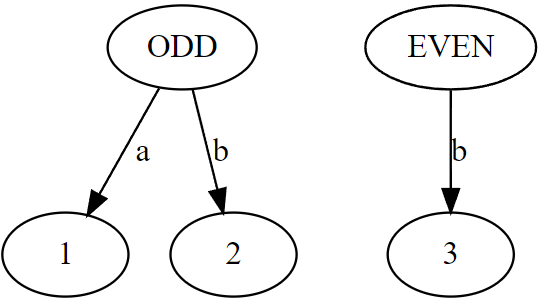
\includegraphics{1.PNG}\\
		请问这个 PAM 里,节点 $3$ 的 $\rm fail$ 指针应该指向哪一个节点?
    \end{frame}
	
    \begin{frame}
        \frametitle{Definition}
		没错,是点 $2$,因为 b 是 bb 的最长回文真后缀。\\
		下面给出完整的图,请读者自行体会(虚线表示 $\rm fail$ 指针)。\\
		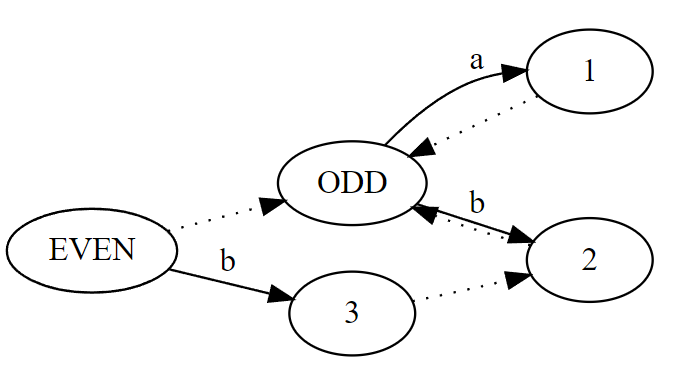
\includegraphics{2.PNG}
    \end{frame}
	
    \begin{frame}
        \frametitle{Extra}
		请注意,$\rm ODD$ 节点实际上有没有 $\rm fail$ 边都没关系,\\
		因为如果一个节点到了 $\rm ODD$ 上是一定能匹配上的(单成一串)\\
		你甚至可以 $\rm fail[ODD] = 114514$ (逃\\
		每个节点还有一个值 $\rm len$ 代表从根走到它产生的回文串的长度。  
    \end{frame}

	\section{Code}
	\begin{frame}
		\frametitle{Variables}
		PAM 的结构和 AC 自动机差不多,就多了个 $\rm len$ 数组。\\
		这里同时给出定义和建造空 PAM 的代码。\\
		由于我 LaTeX 出锅了,这里就直接去 VSC 看吧,很抱歉 /ll\\
		$\rm len[1]$ 一定要初始化为 $-1$!\\
		因为根据单个字符串长度为 $1$ 倒推回去那就是 $1-2=-1$!\\
		(每加一个字符长度加 $2$)
	\end{frame}

	\begin{frame}
		\frametitle{GetFail}
		这玩意很简单,就是不断跳 $\rm fail$,直到能匹配上为止。
	\end{frame}
	
	\begin{frame}
		\frametitle{Insert}
		(对着代码讲)
	\end{frame}
	
	\section{Time Complexity}
	\begin{frame}
		\frametitle{Provement}
		注意到这就是让我们求跳 $\rm fail$ 会跳多少次。  
		很简单:每插入一个节点高度 $+2$,每跳一次 $\rm fail$ 高度 $-2$。\\  
		总共 $n$ 个字符时间复杂度就是 $\mathcal{O}(n)$
	\end{frame}

	\section{Exercise}
	\begin{frame}
		\frametitle{P5496}
		板子题,不多说
	\end{frame}

	\begin{frame}
		\frametitle{P3469}
		先建出 PAM。  
		\pause
		然后我们 倒序循环 每个节点(相当于自底向上遍历 PAM)\\  
		每到一个节点就统计贡献,然后把它 $\rm fail$ 指针指向的节点的 $\rm cnt$ 加上这个节点的 $\rm cnt$\\
		为什么呢?\\  
		设该节点为 $x$, 节点 $x$ 所代表的字符串为 $\rm str_x$,则 $\rm str_x$ 包含 $\rm str_{fail_x}$。\\
		所以要同步更新 $\rm cnt_{fail_x}$。
	\end{frame}

	\begin{frame}
		\frametitle{P1659}
			先建回文自动机,然后自底向上遍历这个 PAM。  \\
			利用一个优先队列来维护一段区间的长度和个数,然后统计贡献时用快速幂即可。
			也可以直接按 $nc \rightarrow 1$ 的顺序跑,都一样。
		\end{frame}

	\begin{frame}
		\frametitle{HDU5785}
		我们先正着跑一遍,记录结果,再 reverse 一下跑一遍。  \\
		记录啥捏?  
		$$
		\begin{aligned}res&=\sum_{j=1}^{n-1}\sum_a\sum_b (j-a)(j+b)\\
			&=\sum\sum\sum (j^2-aj+bj-ab)\\
			&=\sum j^2c_ac_b-c_bs_aj+c_as_bj-s_as_b
		\end{aligned}
		$$
		其中,$c_a$ 代表 $a$ 的个数, $s_a$ 代表 $\sum a$,$c_b,s_b$ 同理。

	\end{frame}

	\begin{frame}
		\frametitle{Others}
		P5555\\
		CF17E\\
		P4287\\
		P4555\\
		以上几道都是练习 PAM 的好题!
	\end{frame}

	\begin{frame}
		\frametitle{The End}
		Thank you for listening!
	\end{frame}
	
\end{CJK}

\end{document}